% Source: printed p. 76; PDF p. 85
Giả sử $\sim$ là một quan hệ tương đương trên $X$. \emph{Thương của $X$ theo $\sim$}, ký hiệu $X/{\sim}$, là tập hợp các lớp tương đương của $\sim$. Theo định nghĩa, với mỗi phần tử $x\in X$, có đúng một lớp tương đương $A$ sao cho $x\in A$. Do đó, ta có thể định nghĩa một hàm $Q:X\to X/{\sim}$, gọi là \emph{hàm thương}, gửi mỗi phần tử $x\in X$ đến lớp tương đương chứa nó. Chú ý rằng với mỗi $y\in X/{\sim}$, tồn tại $x\in X$ sao cho $Q(x)=y$; ta gọi $x$ là một \emph{đại diện} của lớp tương đương $y$.

\noindent\textbf{Ví dụ 3.3.1.2.} Cho $\mathbb Z$ là tập hợp các số nguyên. Định nghĩa một quan hệ $R\subseteq\mathbb Z\times\mathbb Z$ bởi
\[R=\{(x,y)\mid\exists n\in\mathbb Z\text{ sao cho }x+7n=y\}.\]
Khi đó $R$ là một quan hệ tương đương, vì $x+7\cdot0=x$ (phản xạ); $x+7n=y$ khi và chỉ khi $y+7(-n)=x$ (đối xứng); và hai đẳng thức $x+7n=y$, $y+7m=z$ cùng suy ra $x+7(m+n)=z$ (bắc cầu).

Một ví dụ về lớp tương đương $A\subseteq\mathbb Z$ của quan hệ này là $A=\{\ldots,\allowbreak-12,\allowbreak-5,\allowbreak2,\allowbreak9,\allowbreak\ldots\}$.

\noindent\textbf{Bài tập 3.3.1.3.} Cho $X$ là tập hợp những người trên Trái Đất. Định nghĩa một quan hệ hai ngôi $R\subseteq X\times X$ trên $X$ như sau: với một cặp người $(x,y)$, đặt $(x,y)\in R$ nếu $x$ quan tâm đến những gì xảy ra với $y$. Hãy giải thích các câu trả lời của bạn:
\begin{enumerate}[label=\alph*.]
\item Quan hệ này có phản xạ không?
\item Nó có đối xứng không?
\item Nó có bắc cầu không?
\item Nếu thay ``quan tâm đến những gì xảy ra với'' bằng ``đã bắt tay với'' thì sao? Quan hệ này có phản xạ, đối xứng, bắc cầu không?
\end{enumerate}
\noindent\textbf{Lời giải 3.3.1.3.}\keepwithnext
\begin{enumerate}[label=\alph*.]
\item Có; ai cũng quan tâm đến những gì xảy ra với chính mình.
\item Không; $x$ có thể quan tâm đến những gì xảy ra với $y$ mà $y$ không quan tâm đến những gì xảy ra với $x$.
\item Không; tôi quan tâm đến bạn, bạn quan tâm đến John, nhưng tôi chẳng quan tâm chút nào đến những gì xảy ra với John: tôi thậm chí không biết anh ấy.
\item Bắt tay có tính đối xứng, nhưng không phản xạ và không bắc cầu.
\end{enumerate}

% Source: printed p. 77; PDF p. 86
\noindent\textbf{Ví dụ 3.3.1.4 (Phân hoạch).} Một quan hệ tương đương trên tập hợp $X$ có thể được xem là một cách phân hoạch $X$. Một \emph{phân hoạch của $X$} gồm một tập hợp $I$, gọi là \emph{tập hợp các phần}, và với mỗi phần tử $i\in I$, một tập con được chọn $X_i\subseteq X$ sao cho hai tính chất sau đúng:
\begin{itemize}
\item Mọi phần tử $x\in X$ đều thuộc một phần nào đó (tức với mọi $x\in X$, tồn tại $i\in I$ sao cho $x\in X_i$).
\item Không phần tử nào có thể nằm trong hai phần khác nhau (tức nếu $x\in X_i$ và $x\in X_j$ thì $i=j$).
\end{itemize}
Cho một phân hoạch của $X$, ta định nghĩa một quan hệ tương đương $\sim$ trên $X$ bằng cách đặt $x\sim x'$ nếu $x,x'$ nằm trong cùng một phần (tức tồn tại $i\in I$ sao cho $x,x'\in X_i$). Các phần trở thành các lớp tương đương của quan hệ này.\ctIIInote{Bản gốc viết “The parts become the equivalence classes”, nhưng hai điều kiện trên vẫn cho phép $X_i=\varnothing$. Để phát biểu này khớp với định nghĩa lớp tương đương khác rỗng, cần bỏ các phần rỗng hoặc giả sử mọi $X_i\ne\varnothing$.} Ngược lại, cho một quan hệ tương đương, ta tạo một phân hoạch của $X$ bằng cách lấy $I$ là tập hợp các lớp tương đương, và với mỗi $i\in I$, lấy $X_i$ gồm các phần tử trong lớp tương đương ấy.

\noindent\textbf{Bài tập 3.3.1.5.} Cho $X,B$ là các tập hợp và $f:X\to B$ là một hàm. Định nghĩa tập con $R_f\subseteq X\times X$ bởi
\[R_f=\{(x,y)\mid f(x)=f(y)\}.\]
\begin{enumerate}[label=\alph*.]
\item Cho $f:\mathbb R\to\mathbb R$ là hàm cosin, $f(x)=\cos(x)$, và $R_f\subseteq\mathbb R\times\mathbb R$ là quan hệ vừa định nghĩa. Tìm $x,y\in\mathbb R$ sao cho $x\ne y$ nhưng $(x,y)\in R_f$.
\item Với một hàm $f$ bất kỳ, $R_f$ có là quan hệ tương đương không?
\item Có thể thu được mọi quan hệ tương đương trên $X$ bằng cách này không (dưới dạng $R_f$ với một hàm nào đó có miền xác định $X$)?
\item Cách nhìn lớp tương đương này có liên quan đến cách nhìn trong Ví dụ 3.3.1.4 không?
\end{enumerate}
\noindent\textbf{Lời giải 3.3.1.5.}\keepwithnext
\begin{enumerate}[label=\alph*.]
\item Đặt $x=0.7$, $y=2\pi+0.7$, trong đó $\pi\approx3.14159$ là tỉ số giữa chu vi và đường kính của một đường tròn.
\item Có; phản xạ vì $f(x)=f(x)$; đối xứng vì nếu $f(x)=f(y)$ thì $f(y)=f(x)$; bắc cầu vì nếu $f(x)=f(y)$ và $f(y)=f(z)$ thì $f(x)=f(z)$.
\item Cho $B=X/{\sim}$ là thương, và $f:X\to B$ là hàm thương gửi mỗi phần tử của $X$ đến lớp tương đương của nó. Theo định nghĩa, hai phần tử $x,y\in X$ tương đương khi và chỉ khi chúng nằm trong cùng lớp tương đương, $f(x)=f(y)$.
% Source: printed p. 78; PDF p. 87
\item Có; các thớ của $f$ tạo thành một phân hoạch. Nghĩa là, ta có thể lấy $B$ là tập hợp các phần, và với mỗi $b\in B$, định nghĩa tập con $X_b\subseteq X$ là thớ $X_b=f^{-1}(b)$. Khi đó, mọi phần tử của $X$ đều nằm trong một phần (một thớ), và không phần tử nào của $X$ nằm trong hai thớ khác nhau.
\end{enumerate}

\noindent\textbf{Bài tập 3.3.1.6.} Lấy một tập hợp $I$ các tập hợp. Nghĩa là, giả sử $I$ là một tập hợp và với mỗi phần tử $i\in I$, bạn được cho một tập hợp $X_i$. Với mỗi hai phần tử $i,j\in I$, nói rằng $i\sim j$ nếu $X_i,X_j$ đẳng cấu. Quan hệ này có là một quan hệ tương đương trên $I$ không?

\noindent\textbf{Lời giải 3.3.1.6.} Có; $\sim$ là một quan hệ tương đương trên $I$. Đây chính là nội dung của Mệnh đề 2.1.2.18.

Bất kỳ quan hệ nào cũng có thể được mở rộng thành một quan hệ tương đương với sự thay đổi nhỏ nhất.

\noindent\textbf{Mệnh đề 3.3.1.7 (Sinh quan hệ tương đương).} \emph{Cho $X$ là một tập hợp và $R\subseteq X\times X$ là một tập con bất kỳ. Tồn tại một quan hệ $S\subseteq X\times X$ sao cho}
\begin{itemize}
\item $S$ là một quan hệ tương đương;
\item $R\subseteq S$;
\item với mọi quan hệ tương đương $S'$ sao cho $R\subseteq S'$, ta có $S\subseteq S'$.
\end{itemize}
Quan hệ $S$ được gọi\ctIIInote{Bản gốc in “The relation $S'$ is called”. Quan hệ vừa được định nghĩa bằng tính nhỏ nhất là $S$; $S'$ là một quan hệ tương đương chứa $R$ tùy ý.} là \emph{quan hệ tương đương được sinh bởi $R$}.

\begin{proof}[Chứng minh]
Gọi $L_R$ là tập hợp mọi quan hệ tương đương trên $X$ chứa $R$. Nói cách khác, mỗi phần tử $\ell\in L_R$ là một quan hệ tương đương, nên $R\subseteq\ell\subseteq X\times X$. Tập hợp $L_R$ khác rỗng, vì $X\times X\subseteq X\times X$ là một quan hệ tương đương chứa $R$. Gọi $S$ là tập hợp các cặp $(x_1,x_2)\in X\times X$ xuất hiện trong mọi phần tử của $L_R$, tức $S=\bigcap_{\ell\in L_R}\ell$. Theo định nghĩa, $R\subseteq S$. Ta chỉ cần chứng minh $S$ là một quan hệ tương đương.

Rõ ràng $S$ phản xạ vì mỗi $\ell\in L_R$ đều phản xạ. Nếu $(x,y)\in S$, thì $(x,y)\in\ell$ với mọi $\ell\in L_R$. Nhưng vì mỗi $\ell$ là một quan hệ tương đương, $(y,x)\in\ell$ cũng đúng, nên $(y,x)\in S$. Điều đó cho thấy $S$ đối xứng. Chứng minh tính bắc cầu tương tự: nếu $(x,y)\in S$ và $(y,z)\in S$, thì chúng đều nằm trong mỗi $\ell$; do đó $(x,z)$ nằm trong mỗi $\ell$, và vì vậy nằm trong $S$.
\end{proof}

% Source: printed p. 79; PDF p. 88
\noindent\textbf{Bài tập 3.3.1.8.} Xét tập hợp $\mathbb R$ các số thực. Vẽ mặt phẳng tọa độ $\mathbb R\times\mathbb R$, đặt các tọa độ là $x,y$. Một quan hệ hai ngôi trên $\mathbb R$ là một tập con $S\subseteq\mathbb R\times\mathbb R$, có thể được vẽ thành một tập hợp các điểm trong mặt phẳng $(x,y)$.
\begin{enumerate}[label=\alph*.]
\item Vẽ quan hệ $\{(x,y)\mid y=x^2\}$.
\item Vẽ quan hệ $\{(x,y)\mid y\ge x^2\}$.
\item Gọi $S_0$ là quan hệ tương đương trên $\mathbb R$ được sinh bởi tập rỗng, theo nghĩa của Mệnh đề 3.3.1.7. Vẽ $S_0$ như một tập con của mặt phẳng.
\item Xét quan hệ tương đương $S_1$ được sinh bởi $\{(1,2),(1,3)\}$. Vẽ $S_1$ trong mặt phẳng. Làm nổi bật lớp tương đương chung của $1$ và $2$.\ctIIInote{Bản gốc viết “the equivalence class containing $(1,2)$”. Quan hệ $S_1$ là trên $\mathbb R$, nên phần tử của một lớp là số thực. Ở đây hiểu là lớp chung chứa $1$ và $2$, tức $\{1,2,3\}$.}
\item Tính chất phản xạ và tính chất đối xứng, từ Định nghĩa 3.3.1.1, có những cách minh họa đẹp trong $\mathbb R\times\mathbb R$; đó là những cách nào?
\item Bạn có thể nghĩ ra một cách minh họa gần đúng cho tính chất bắc cầu không?
\end{enumerate}

\noindent\textbf{Lời giải 3.3.1.8.}\keepwithnext
% Native plots checked against supplied PDF p. 79–81; grid ranges retained.
\providecommand{\ctIIIparabolagrid}{\foreach \x in {-4,...,4}{\draw[thin] (\x,-5)--(\x,20);\node[below,font=\scriptsize]at(\x,-5){$\x$};}\foreach\y in{-5,0,5,10,15,20}{\draw[thin](-4,\y)--(4,\y);\node[left,font=\scriptsize]at(-4,\y){$\y$};}}
\providecommand{\ctIIIsquaregrid}{\foreach \x in {-4,...,4}{\draw[thin](\x,-5)--(\x,5);\node[below,font=\scriptsize]at(\x,-5){$\x$};}\foreach\y in{-5,...,5}{\draw[thin](-4,\y)--(4,\y);\node[left,font=\scriptsize]at(-4,\y){$\y$};}}
\begin{enumerate}[label=\alph*.]
\item
\begin{center}\begin{tikzpicture}[x=.65cm,y=.16cm]\ctIIIparabolagrid\draw[gray,domain=-4:4,samples=100]plot(\x,{\x*\x});\end{tikzpicture}\end{center}
% Source: printed p. 80; PDF p. 89
\item
\begin{center}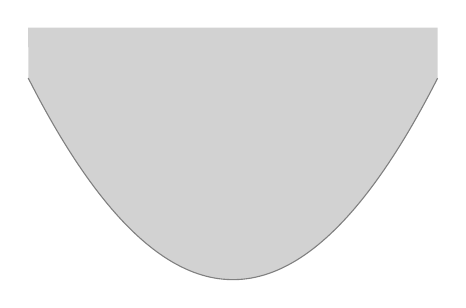
\begin{tikzpicture}[x=.65cm,y=.16cm]
\fill[gray!35](-4,20)--(4,20)--(4,16)--plot[domain=4:-4,samples=100](\x,{\x*\x})--cycle;
\ctIIIparabolagrid\draw[gray,domain=-4:4,samples=100]plot(\x,{\x*\x});\end{tikzpicture}\end{center}
\item
\begin{center}\begin{tikzpicture}[x=.65cm,y=.4cm]\ctIIIsquaregrid\draw[gray](-4,-4)--(4,4);\end{tikzpicture}\end{center}
% Source: printed p. 81; PDF p. 90
\item
\begin{center}\begin{tikzpicture}[x=.65cm,y=.4cm]\ctIIIsquaregrid\draw[gray](-4,-4)--(4,4);\foreach\x/\y in{1/2,1/3,2/1,2/3,3/1,3/2}{\fill(\x,\y)circle(2pt);}\end{tikzpicture}\end{center}
\item Một quan hệ $R$ phản xạ nếu đồ thị của nó trong mặt phẳng $(x,y)$ chứa đường thẳng $y=x$. Quan hệ đó đối xứng nếu đồ thị của nó đối xứng qua đường thẳng $y=x$.
\item Tôi không nghĩ ra được một cách hay.
\end{enumerate}

\noindent\textbf{Bài tập 3.3.1.9.} Cho $X$ là một tập hợp và xét quan hệ rỗng $R=\varnothing\subseteq X\times X$.
\begin{enumerate}[label=\alph*.]
\item Quan hệ tương đương $\sim$ được sinh bởi $R$ là gì (gọi là \emph{quan hệ tương đương tầm thường} trên $X$)?
\item Hàm thương $X\to X/{\sim}$ có luôn là một đẳng cấu không?
\end{enumerate}
\noindent\textbf{Lời giải 3.3.1.9.}\keepwithnext
\begin{enumerate}[label=\alph*.]
\item Đó là quan hệ phản xạ nhỏ nhất $R:=\{(x,x)\mid x\in X\}$.
\item Có. Ta có $x\sim y$ khi và chỉ khi $x=y$, nên mỗi lớp tương đương chứa đúng một phần tử.
\end{enumerate}

\noindent\textbf{Bài tập 3.3.1.10.} Xét quan hệ hai ngôi $R=\{(n,n+1)\mid n\in\mathbb Z\}\subseteq\mathbb Z\times\mathbb Z$.
% Source: printed p. 82; PDF p. 91
\begin{enumerate}[label=\alph*.]
\item Quan hệ tương đương $\sim$ được sinh bởi $R$ là gì?
\item Có bao nhiêu lớp tương đương?
\end{enumerate}
\noindent\textbf{Lời giải 3.3.1.10.}\keepwithnext
\begin{enumerate}[label=\alph*.]
\item Với mọi hai phần tử $m,n\in\mathbb Z$, ta có $m\sim n$. Vì sao? Hãy nghĩ xem chuyện gì xảy ra nếu $m,n$ cách nhau $k$, tức $|m-n|=k$. Nếu $k=0$, ta có $m\sim n$ do tính phản xạ; nếu $k=1$, ta có $m\sim n$ theo định nghĩa và tính đối xứng. Ta có được trường hợp $k=2$ nhờ tính bắc cầu. Sau đó, lại dùng tính bắc cầu để có trường hợp $k=3$; cứ tiếp tục như vậy, ta thấy $m\sim n$ bất kể khoảng cách $k$.
\item Có một lớp tương đương.
\end{enumerate}

\noindent\textbf{Bài tập 3.3.1.11.} Giả sử $N$ là một mạng (hệ thống các nút và cạnh). Cho $X$ là tập hợp các nút của mạng và $R\subseteq X\times X$ là quan hệ sao cho $(x,y)\in R$ khi và chỉ khi có một cạnh nối $x$ với $y$.\footnote{Từ viết tắt \emph{iff} trong tiếng Anh có nghĩa là ``khi và chỉ khi''. Ở đây, ta nói cặp $(x,y)$ nằm trong $R$ khi và chỉ khi tồn tại một mũi tên nối $x,y$.}
\begin{enumerate}[label=\alph*.]
\item Quan hệ tương đương $\sim$ được sinh bởi $R$ là gì?
\item Thương $X/{\sim}$ là gì?
\end{enumerate}
\noindent\textbf{Lời giải 3.3.1.11.}\keepwithnext
\begin{enumerate}[label=\alph*.]
\item Nút $x$ tương đương với nút $y$ khi và chỉ khi ta có thể đi từ $x$ đến $y$ dọc theo một số hữu hạn cạnh (kể cả không đi qua cạnh nào nếu $x=y$). Nói cách khác, nếu các nút là địa chỉ đường phố trong một thành phố và mỗi cạnh giống như một con đường, thì hai địa chỉ tương đương khi một người đi bộ có thể đi từ địa chỉ này đến địa chỉ kia.
\item Đó là tập hợp các ``thành phần liên thông'' của mạng. Hãy hình dung một thành phần liên thông như một hòn đảo trong mạng. Một người đi bộ có thể đi từ bất cứ đâu trên đảo đến bất cứ chỗ nào khác trên đảo, nhưng không thể ra khỏi đảo.
\end{enumerate}
